\section{Security Isolation}
\label{sec:linux:security}

\issuedone{1.1.d}{describe the security isolation story for Linux hosts}
\graphene{} separates OS features from security isolation.
This section explains the Linux host design for isolating mutually untrusting applications, with a reduced attack surface for protecting Linux kernels.
The discussion starts with the security guarantees and threat model, followed by the technical details of security isolation on a Linux host.



\subsection{Security guarantees}

The security isolation model of \graphene{} ensures that mutually-untrusting applications cannot interfere with each other.
A goal of \graphene{} is to provide security isolation with comparable strength as
running applications in separate VMs.
When running two unrelated applications on the same machine,
the security requirement
of the OS involves not only blocking unauthorized access under normal circumstance,
but also preventing an application
from maliciously exploiting OS vulnerabilities to attack the other application.
Because a modern OS, such as Linux or Windows, contains a rich of features and APIs,
it is difficult to eliminate OS vulnerabilities
or even just to verify whether an OS contains any vulnerabilities. 
A Linux container~\cite{lxc}
does provide a separate OS view for each application,
but still relies on the correctness of the whole Linux kernel to enforce security isolation.
On the other hand, a VM or a \libos{}
isolates the whole OS kernel or a part of the kernel in an unprivileged guest space
for each application.
The security isolation model prevents
any vulnerabilities inside the VM or the \libos{} from compromising the host kernel and other applications.



\graphene{} enforces security isolation %between applications
by separating 
backward-compatible OS features from security mechanisms.
A Linux kernel exports a wide range of \linuxapis{},
either as a legacy of previous kernels or as new programmability features. % of newer kernels.
By implementing OS features in a \libos{},
\graphene{} reduces the attack surface of a Linux kernel
to a small amount of \linuxapi{} corner cases.
%to implement \thehostabi{}.
%If a machine only runs applications in \graphene{},
%a Linux developer can try to carve out a minimal Linux kernel, containing only features needed by the Linux PAL.
A reduced attack surface
eliminates majority of execution paths inside a Linux kernel in which a malicious application can explore for vulnerabilities.
The complexity of Linux features and APIs exported by a \libos{} is unrelated with the attack surface of the host kernel,
unless the \libos{} asks for additional \hostapis{}.
A Linux developer can even carve out a minimal Linux kernel with only the features needed by the Linux PAL,
similar to shrinking a Linux kernel to a microkernel.
Otherwise, \graphene{} depends on the host security mechanisms to restrict a \libos{} from accessing unauthorized \linuxapis{} and resources upon an unmodified Linux kernel.





The Linux PAL installs a {\bf \linuxapi{} filter} and a {\bf reference monitor}
for restricting the \linuxapis{}, files, RPC streams, and network addresses
accessed by a \picoproc{}.
The Linux PAL requires \hostsyscallnum{} \linuxapis{} in total
for implementing both required and optional \hostapis{}.
A \linuxapi{} filter, such as the Linux \seccomp{} filter~\cite{seccomp},
can restrict the \linuxapi{} access of an application
to only a small subset of all the \linuxapis{}, with additional constraints on the parameters and optional flags permitted for each \linuxapi{}.
%The \linuxapi{} filter
%forbids an application from invoking any \linuxapis{}
%that will interfere other \picoproc{} or increase the risk of exploitation in the host kernel.
A reference monitor further examines the arguments of permitted \linuxapis{} to restrict the host resources accessed by an application, based on security policies configured in a manifest file~\cite{hunt07rethink}.
The \linuxapi{} filter and the reference monitor
significantly limit the ability of an untrusted \graphene{} \picoproc{} to interfere with the rest of the system,
preventing the risk of exposing any unknown vulnerabilities
on a kernel path never exercised by the \linuxapi{} footprint of \graphene{}.



\graphene{} contributes a multi-process security model 
based on a {\bf sandbox},
or a set of mutually-trusting \picoprocs{} running inside an isolated container.
The reference monitor permits picoprocesses within the same sandbox
to communicate over RPC streams,
allowing the \libos{} to share and coordinate any states
to create an unified OS view.
If two \picoprocs{} belong to different sandboxes,
the reference monitor will block any attempt of connecting RPC streams
between the \picoprocs{}
The access control over RPC streams
enforces an all-or-nothing security isolation model:
either two \picoprocs{} are in the same sandbox and share all the \libos{} states; or they are separated in two sandboxes and share nothing.
Even though the \libos{} instance can span its state across multiple \picoprocs{},
a host kernel needs not to examine the accesses to shared \libos{} states, but still enforces security isolation between sandboxes.




Files and network addresses
are the only host resources allowed to be shared across sandboxes,
using well-studied, explicit rules.
For sharing files, the reference monitor restricts the file access of a \picoproc{}
within a few host file or directories,
creating a restricted view of the local file system
(close to Plan 9's unionized file system views~\cite{pike90plan9}).
The file rules
in a manifest are similar to the policies of a {\bf AppArmor profile}~\cite{apparmor};
for each permitted file or directory,
a developer specifies the URI prefix and the permitted access type, either as read-only or readable-writable. %, within the target file or directory.
For sharing network addresses,
the reference monitor restricts a \picoproc{} from connecting through a local address or connecting to a remote address,
using {\bf iptables-like firewall rules}~\cite{iptablesman}.
Each network rule in a manifest
specifies the local or remote IP address and port range that a \picoproc{} is permitted to bind or connect a network socket.
The rules in a manifest file
specify a minimal list of files and network addresses that a \picoproc{} needs to access, and are largely based on existing security policies (e.g., AppArmor profiles, firewall rules).





\paragraph{Threat model (details).}
When running on a normal Linux host (without SGX or other security hardware), \graphene{} assumes a trusted host kernel and reference monitor.
All the components inside the kernel space, including the \code{gipc} kernel module for bulk IPC, and the reference monitor,
are fully trusted by the other parts of the host kernel and the \graphene{} \picoprocs{}.
%which mediates all system calls with effects outside of a picoprocess's address space,
%such as file {\tt open} or network socket {\tt bind} or {\tt connect}.
On the other hand,
the host Linux kernel does not trust the \picoproc{}, including the Linux PAL, a \thelibos{} instance, \glibc{}, and the application.
The \linuxapi{} filter and reference monitor
initialized before an application starts running
defend the whole host kernel from malicious \linuxapis{} invoked by a \picoproc{}.



All the components running within a \picoproc{}, including the Linux PAL, the \libos{} (\thelibos{}), \glibc{} libraries, and the application,
mutually trust each other. %, because all these components
%execute in the same guest address space.
Without internal sandboxing, the Linux PAL or \thelibos{}
cannot protect its internal states or control flows from an application.
Although some scenarios might require protecting the PAL or \thelibos{}
from the application,
\graphene{} only restricts the adversary
within a \picoproc{};
in other word, an adversary
only compromises the \libos{} in the same \picoproc{},
but can never interfere the host kernel 
or other unrelated \picoprocs{}.



For a multi-process application,
\graphene{} assumes that the \picoprocs{} 
%launched by the same application instance
running inside the same sandbox
trust each other and that all untrusted code run in sandboxed \picoprocs{}.
\graphene{} assumes the adversary can run arbitrary code inside
one or multiple \picoprocs within a sandbox.
The adversary can exploit any vulnerabilities in the \libos{}
or IPC protocol,
to propagate the attack to other \picoprocs{}.
\graphene{} ensures that
the adversary cannot interfere with any victim \picoprocs{}
in a separate sandbox.
A sandbox strictly isolates the coordination of \thelibos{} instances;
%if the only shared kernel abstractions are byte streams and files, 
the reference monitor ensures
that there is no writable intersection between sandboxes, so that
the adversary cannot interfere with any victim \picoprocs{}.


%%% The only processes allowed to run as standard kernel processes (non-\graphene{}) 
%%% are the reference monitor and
%%% system administration utilities that need more kernel interfaces than the \pal{} ABI provides.
%%% Ensuring that a collaborating picoprocess correctly implements
%%% some function (such as receiving a signal),
%%% as well as preventing exploitation of vulnerabilities in picoprocesses
%%% are beyond the scope of this work.

\graphene{} reduces the attack surface of the host Linux kernel, but does not change the trusted computing base; however, reducing the effective \linuxapi{} table size of a \picoproc{} does facilitate adoption of a smaller host kernel.
This thesis leaves the creation of a smaller host kernel for future work.

\subsection{System call restriction}
\label{sec:linux:security:syscall-restriction}


\graphene{} reduces the host ABI to \palcallnum{} calls
and the Linux \linuxapi{} footprint to \hostsyscallnum{} \linuxapis{}.
To reduce the effective attack surface to a Linux host,
the Linux host restricts a \picoproc{} from accessing any \linuxapis{} that are not part of the ordinary footprint of a Linux PAL.
The \linuxapi{} restriction on Linux focuses on blocking most of the \linuxapis{}
that interferes with other processes.
The remaining permitted \linuxapis{} with external effects are checked by 
the reference monitor (see Section~\ref{sec:linux:security:ref-monitor}).
 
%% dp: Meh
%%% Any picoprocess implementation 
%%% must restrict access to the host system call table,
%%% generally by blocking system calls in the host kernel~\cite{porter11drawbridge}
%%% or using {\tt ptrace}~\cite{xax}.


%The \pal{} is a host-provided library which implements \palcalls{} generic kernel ABIs,
%implemented using 
%These native system calls include {\tt ioctl} with 5 opcodes exclusively used by \graphene{} kernel extensions.

%This section describes how we adapt recent Linux sandboxing techniques 
%to \graphene{}.


%all allowed system calls with potentially external effects.

%%% For instance, an attempt to open a file will be checked by the reference monitor
%%% to see if the file is included in the sandbox definition, specified in the manifest
%%% with required permissions.
%%% Once the file handle is open, the \pal{} is then allowed to issue an {\tt mmap} or {\tt read}
%%% on the handle, as this operation can only affect the picoprocess address space
%%% or  file, which was already checked.

%Because the \pal{} is in the same address space as the application code, it is not
%trusted to enforce any security policies, and our threat model assumes that
%the \pal{} can be compromised by the adversary.
%Thus, the host kernel 
%only permits system calls that appear in the \pal{}'s source code and, through the reference monitor, further inspects calls that can have external effects.

%\begin{figure}[t!]
%\centering
%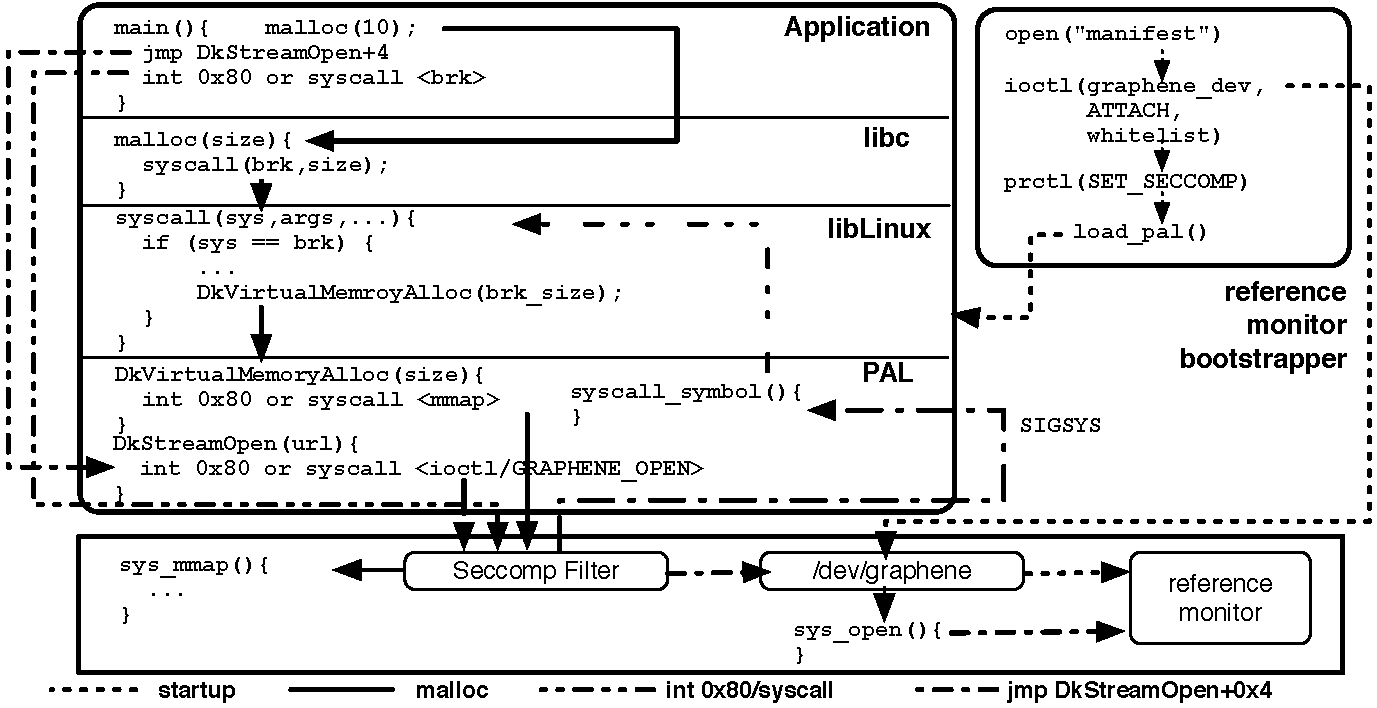
\includegraphics[width=\linewidth]{syscall-restriction.pdf}
%\footnotesize
%\caption[System call restriction approach in sysname{}]
%{System call restriction approach. The reference monitor loads policies into the LSM at startup.  A \graphene{} application requests OS services in three different ways. 
%In the normal case (first line of {\tt main}), {\tt malloc} is invoked causing the invocation of {\tt brk} ({\tt libLinux}) and {\tt mmap} in the \pal{}. In the second line, the application jumps to an address in \pal{}, which is permissible.
%Files are accessed through {\tt ioctl} to {\tt /dev/graphene} and checked by reference monitor.
%The third line invokes {\tt brk} with an {\tt int} instruction, which is redirected to the {\tt libLinux} function.}
%\label{fig:graphene:syscall-restriction}
%\end{figure}



\issuedone{1.3.d}{extend the discussion of \seccomp{} filter}
\graphene{} restricts the host \linuxapis{} 
using a \seccomp{} (SECure COMPuting) filter~\cite{seccomp}. The feature of \seccomp{} filters is introduced to the Linux kernels since 2.6.12.
% a recent Linux system call filtering mechanism, called 
A \seccomp{} filter allows a Linux process to install an immutable Berkeley Packet Filter (BPF) program
that specifies allowed \linuxapis{}, as well as specifies
the consequence of invoking certain \linuxapis{}, such as creating a \code{ptrace} event or raising a \code{SIGSYS} signal.
The BPF grammar is rich enough to filter scalar argument values,
such as only permitting specific opcodes for \syscall{ioctl},
as well as filter certain register values, such as blocking \linuxapis{} from program counters outside of the Linux PAL.
%This feature is particularly salient in the case of {\tt ioctl},
%where the \pal{} uses 5 out of over 400 opcodes for our bulk IPC module and sandbox creation;
%our BPF rules will block any other {\tt ioctl} opcode.
The current \seccomp{} filter installed by the Linux PAL contains \seccomplines{} lines of straightforward BPF macros.  %Experiments show that adding more precise argument checks has no significant impact on \linuxapi{} latency.
Once a \seccomp{} filter is installed in a process,
the filter intermediates
every \linuxapis{} from the process and its future children, and guarantees the processes can never bypass the restriction.
The Linux PAL uses \code{SIGSYS} signals to capture rejected \linuxapis{},
and can either terminate the whole application or
redirect the \linuxapi{} to \thelibos{}.
The consecutive steps of \linuxapi{} redirection are described in Section~\ref{sec:libos:syscall-redirection}.



Despite the straightforwardness of \seccomp{} filters, developing a robust filter for a \graphene{} application presents several challenges.
First, the initially-installed filter must prevent consecutive \picoprocs{}
from reverting the \linuxapis{} restriction.
Since
\seccomp{} filters are installed using the \syscall{prctl} \linuxapi{},
blocking \syscall{prctl} in a filter prevents further changes to the \linuxapi{} restriction rules (there is no other usage of \syscall{prctl} in the Linux PAL).
Second, 


Unfortunately, the logic to check for allowed paths network addresses cannot be implemented 
as a seccomp rule, because it involves reading user memory of unknown sizes. 
In order to avoid the overhead of trapping to the reference monitor on 
every use of {\tt open}, {\tt stat}, {\tt bind} or {\tt connect} system calls, we instead 
force picoprocess to only use {\tt ioctl} system call to \graphene{} special device ({\tt /dev/graphene}) as alternative interface these system calls. Direct access to these system calls are banned by seccomp filter.
%extend AppArmor~\cite{apparmor} 
%to enforce file system isolation in the kernel.

In order to reduce the impact of bugs in the reference monitor,
the reference monitor itself runs with a seccomp filter,
blocking unexpected system calls.

\paragraph{Static Binaries.} 
For compatibility with statically linked binaries, which 
compile in system call instructions,
we leverage seccomp to redirect these calls 
back to {\tt libLinux}.  
For system calls that could also be issued by the \pal{},
we augment our BPF rules with program counter-based filters.
In other words, an {\tt open} system call with a return PC address inside the \pal{} 
will be sent to the reference monitor for further inspection;
an {\tt open} system call with any other return PC address generates 
a {\tt SIGSYS} and is ultimately relayed back to {\tt libLinux}.
Thus, {\tt libLinux} can catch and differentiate application-issued system calls
from those that could also be issued by the \pal{}.
We hasten to note this feature is only for backward compatibility,
not security.


\subsection{Reference monitor}
\label{sec:linux:security:ref-monitor}

The \graphene{} reference monitor on a Linux host
is implemented using {\tt ioctl} system call to a special device {\tt /dev/graphene}.
A picoprocess is restricted by seccomp filter~\cite{seccomp} to use any {\tt open} or socket {\tt connect} and {\tt bind} system calls.
It must use the \graphene{} special device to open or create streams,
so the file paths or network addresses can be checked against the sandbox rules.
The kernel module as the driver of the \graphene{} special device can coexist with any LSM such as \emph{AppArmor} or \emph{SELinux}.


When a new picoprocess is launched by the reference monitor, it begins execution in 
a new sandbox.  
Child picoprocesses may either inherit their parent's sandbox, 
or can be started in a separate sandbox
--- specified by a flag to the picoprocess creation ABI.
A parent may specify a subset of its own file system view 
when creating a child, but may not request access to new regions of the 
host file system. 
%The restrictive policy enforced on the child will be written in a new manifest file generated by the parent, and the policy will be checked by the reference monitor.
The child may also issue an {\tt ioctl} call to 
dynamically detach from the parent's sandbox. The reference monitor prevents byte stream creation 
across sandboxes.
%among picoprocesses
%that are not in the same sandbox.
%and restricts external connections to remote URIs according to firewall rules in the manifest.
When a process detaches from a sandbox --- effectively splitting the sandbox ---
the reference monitor closes
any byte streams that could bridge the two sandboxes.


\begin{comment}
We hasten to note that program counter filtering
is only provided for backwards compatibility, not security.
An attacker can compromise the \pal{}, so system policies are enforced
externally by the reference monitor.


Dynamically redirecting system calls to {\tt libLinux} is 
less efficient than dynamically linking against
the \graphene{} libc or statically compiling {\tt libLinux} into the application.
The overhead of dynamic redirection comes from 
transferring control to the kernel, then back to 
the \pal{}, and then to {\tt libLinux}.
We leave exploration of more efficient alternatives for future work,
such as redirecting the hardware system call table to {\tt libLinux}
on a host system like Dune~\cite{belay12dune},
or dynamically rewriting parts of the static binary~\cite{hunt99detours}.
\end{comment}

\paragraph{Example.}
Figure~\ref{fig:graphene:syscall-restriction} illustrates three possible situations. 
%% An unmodified Linux application is dynamically linked against the 
%% \graphene{} {\tt libc}, 
%% which then dynamically links its system calls from {\tt libLinux},
%% which in turn links in the host kernel ABI from the \pal{}.
%% The application requests OS functionality in three ways.
An unmodified application first invokes the {\tt libc} function {\tt malloc}, which issues 
a {\tt brk} system call to {\tt libLinux}, which requests memory 
from the host via a {\tt Dk\-Virtual\-Memory\-Alloc} \pal{} call,
which ultimately issues an {\tt mmap} host system call.
The {\tt mmap} host system call is allowed by seccomp because it only 
affects the picoprocess's address space.
The second line of the application jumps to the \pal{} instruction that issues
an {\tt open} system call.
From a security perspective, this is permissible,
as it is isomorphic to \pal{} functionality.
In practice, this could cause
corruption of {\tt libLinux} or application data structures,
but the only harm is to the application itself. 
Because this system call involves the file system, the reference monitor LSM first checks if the file to be opened is included in the sandbox definition (manifest) before allowing  the {\tt open} system call in the kernel.  
Finally, the application uses inline assembly to issue a {\tt brk} system call;
%in an attempt to obtain I/O port privilege; 
because this system call was not issued by the \pal{},
seccomp will redirect this call back to the \pal{},
which then calls the {\tt libLinux} implementation.

\paragraph{Process-specific Isolation.} 
Sandbox creation in \graphene{} can provide
more options than virtualization, to reflect the security policy of applications at any timing,
in the granularity of picoprocess. 
A picoprocess can voluntarily detach itself from the current sandbox, dropping its privileges,
after finishing security-sensitive operations.
If a picoprocess decides one of its children is not trustworthy, it may also start the child under a restricted manifest,
or promptly shut down RPC streams to stop sharing OS states.
The picoprocess that moves to a separate sandbox will have a restrictive view of the filesystem, and no coordination with the previous sandboxes.
In section~\ref{sec:graphene:eval}, we describe an experiment that improves security isolation of Apache web server without sacrificing functionality.

\paragraph{Reference monitor.}
The reference monitor is a trusted process that runs on the host system.
\graphene{} applications are launched by the reference monitor,
which instantiates the seccomp filter and traces all children
to check host system calls that could have external effects.
The reference monitor interposes using ptrace events, 
which can be raised for specific system calls by seccomp.
We ensure that all processes created within a sandbox are traced
by setting the {\tt PTRACE\_O\_TRACEseccomp{}} option on all newly created picoprocesses
in the sandbox.

%% from bpjain:
% We have to set the option PTRACE\_O\_TRACESECCOMP on new children
% using ptrace(PTRACE\_SETOPTIONS) and we get the event as
% PTRACE\_EVENT\_SECCOMP whenever a syscall that is Traced is called.
% It happens before the grandchild starts running. We get the
% notification of creation of grandchildren by setting ptrace option
% PTRACE\_O\_TRACECLONE on the child(i.e., parent of grandchild).  I
% need to monitor every fork/clone (only clone since pal only calls
% clone). I get this event even if fork/clone is just allowed.  And
% the event that arrives on clone/fork is completely different from
% seccomp event. Thats a ptrace event too.. but we get
% PTRACE\_EVENT\_CLONE whenever a clone is done by a child on which
% PTRACE\_O\_TRACECLONE option was set.

Each application includes a \emph{manifest file}, which specifies restrictions,
including network firewall rules and subsets of the host file system sandboxed
applications are permitted to access.  The reference monitor enforces these
rules by interposing on all system calls involving file paths or remote network addresses.
%\fixmedp{Revise if we can do something smarter; 2x check implementation status before submission}.

%% dp Sadface :(
\paragraph{Privilege.~} 
Although the reference monitor is trusted, it does not run 
with administrative privilege.
Linux 3.5, which we use as our host kernel, 
introduced the {\tt NO\_NEW\_PRIVS} bit, which permits
a non-privileged process to impose sandboxing restrictions on a child.
%Ubuntu back-ported this feature to Linux 3.2, which we use as our host kernel.
This flag prevents a process from acquiring root privilege, % (e.g., via executing a {\tt setuid} binary),
is inherited by all descendant processes,
and cannot be disabled.

\paragraph{Creating New Sandboxes.~} We add a \pal{} call which
permits a picoprocess to request that it be moved into a new sandbox.
This call, as well as file system path checks, are implemented
as extensions to the  AppArmor LSM~\cite{apparmor}.
%We modify \sandboxmodlines{} lines in the
%to implement this call,
The new sandbox call closes any open stream handles that cross sandbox boundaries;
mediate path lookups;
and create a new broadcast stream for multi-process
 coordination (\S\ref{sec:graphene:namespaces:blocks}).
%The reference monitor also interposes on this call so that it can 
%mediate future stream creation.

To securely apply seccomp filtering we leveraged the fact that all
\graphene{} processes have the same parent and also the new
{\tt NO\_NEW\_PRIVS} bit introduced for Linux processes starting kernel
version 3.5. This bit can be set by any process, is inherited across
{\tt fork}, {\tt clone}, and {\tt execve}, and cannot be unset by
children processes. Thus, we set the {\tt NO\_NEW\_PRIVS} bit in the initial
\graphene{} process and apply seccomp filters allowing only system calls
with corresponding functions in the \pal{}. As a result all \graphene{}
processes will inherit the filters and cannot relax or bypass it.



%which reduces the kernel
%system call API surface to user-level processes. This mechanism allows
%a process to specify a whitelist filter for system calls, which is
%implemented as a Berkeley Packet Filter (BPF) program. The invocation
%of a disallowed system call causes the application to throw a {\tt SIGSYS}
%signal, which can be caught by a registered handler provided by the
%application. In \graphene{} we registered this handler at the \pal{}.


%\graphene{} applications rely on an OS loaded as a library to request
%system services. As most of traditional applications, \graphene{}
%processes do not normally issue system calls directly: they invoke
%wrapper functions from a \graphene{}-compliant version of libc, which
%allows for portability, security (parameters are limited and checked)
%and easiness of programming. However, while standard libc functions
%directly invoke the kernel system call themselves, our modified
%version of libc wrappers invoke functions from another library which
%represents the OS, libLinux (Figure \ref{fig:graphene:syscall-restriction}). A
%\graphene{} application can access all necessary system functionality
%through libLinux, which invokes corresponding system call functions at
%the \pal{}, also loaded as a library with a
%\graphene{} process. The \pal{} is the layer responsible for directly
%invoking system calls at the kernel. As discussed in \S\ref{sec:graphene:impl} the \pal{} provides \graphene{} applications with a
%subset of the kernel system call interface.\graphene{} applications rely
%on an OS loaded as a library to request system services.
%
%Even though we expect most of \graphene{} applications to leverage libc
%wrappers, we need to address applications that need to invoke system
%calls directly. Applications might need to bypass a library such as
%libc because some needed wrappers are not provided (there are no
%wrappers in libc for module and NUMA related system calls), or the
%wrapper does not meet the programmer’s needs. \graphene{} applications
%that need to perform direct invocation of system calls run unmodified
%as long as the system calls invoked are provided by the libos{l{}. We
%do not consider this a security violation; even though the application
%would be risking not functioning according to the libosaradigm for
%bypassing the \pal{}, all potential damage would be confined in the
%misbehaving application itself.  However, we do not allow the direct
%invocation of a system call that does not have a corresponding
%function in the libosnd \pal{}. In Figure \ref{fig:graphene:syscall-restriction}
%we illustrate these three situations. We have a \graphene{} application
%loaded with three libraries: a \graphene{}-compliant libc, libLinux
%representing the library OS with functions for a selected number of
%system calls, and the \pal{} which actually invokes host kernel system
%calls. The illustrated application requests three different types of
%OS functionality. It first invokes a function from libc, then it
%directly invokes a system call whose functionality is provided by the
%\pal{}, and third it attempts to directly invoke a system call not
%present in the \pal{}, which is not allowed by \graphene{}.

%We enforce system call restriction by leveraging seccomp Linux system
%call filtering mechanism~\cite{seccomp}, which reduces the kernel
%system call API surface to user-level processes. This mechanism allows
%a process to specify a whitelist filter for system calls, which is
%implemented as a Berkeley Packet Filter (BPF) program. The invocation
%of a disallowed system call causes the application to throw a {\tt SIGSYS}
%signal, which can be caught by a registered handler provided by the
%application. In \graphene{} we registered this handler at the \pal{}.
%
%To securely apply seccomp filtering we leveraged the fact that all
%\graphene{} processes have the same parent and also the new
%{\tt NO\_NEW\_PRIVS} bit introduced for Linux processes starting kernel
%version 3.5. This bit can be set by any process, is inherited across
%{\tt fork}, {\tt clone}, and {\tt execve}, and cannot be unset by
%children processes. Thus, we set the {\tt NO\_NEW\_PRIVS} bit in the initial
%\graphene{} process and apply seccomp filters allowing only system calls
%with corresponding functions in the \pal{}. As a result all \graphene{}
%processes will inherit the filters and cannot relax or bypass it.


%\begin{figure}
%\begin{centering}
%\includegraphics[width=2.0in\textwidth]{figures/syscall_restriction.png}
%\footnotesize
%\caption{System call restriction approach. \graphene{} application requesting OS services. The {\tt printf} function is handled by a wrapper function at our modified version of libc., which invoked a corresponding syscall function at libLinux, the library OS.This function invokes a system call function at the \pal{}, which actually invokes kernel system calls. The application also directly invokes two system calls and the last invocation is prohibited.
%\label{fig:syscall_restriction}
%\end{centering}
%\end{figure}

%\end{comment}
